\chapter{Background}
\minitoc

% \section{Transformer}\label{sec:transformer}

% \subsection{Model Architecture}

% \subsection{Scaled Dot\textendash Product Attention}

% \subsection{Multi\textendash Head Attention}

% \subsection{Self\textendash Attention and Multi\textendash Head Self\textendash Attention}

% \subsection{Feed Forward Network}

% \section{Vision Transformer (ViT)}

% \section{Lightweight ViT}

\section{Recommendation Systems}\label{sec:recommendation-systems}
A recommendation system is an artificial intelligence (AI) technology that provides users with recommendations for items that they may be interested in using Big Data and machine learning techniques. 

Recommender systems undergo training to understand the preferences, earlier decisions, and attributes of the user and products using their past interactions which includes impressions, clicks, purchases, and ratings. Recommender systems are usually used by content and product providers to suggest items to users that they may like based on their profile and preferences.

\section{Types of Recommendation Systems}\label{sec:types-of-recommendation-systems}
There are many four types of recommendation systems:
\subcaption{Collaborative filtering}\label{subsec:collaborative-filtering}
Collaborative filtering is a technique that can filter out items that a user might like on the basis of reactions by similar users. It works by searching a large group of people and finding a smaller set of users with tastes similar to a particular user. It looks at the items they like and combines them to create a ranked list of suggestions. This technique is based on the idea that people who agreed in the past will agree in the future.
\begin{figure}[htbp]
    \centering
    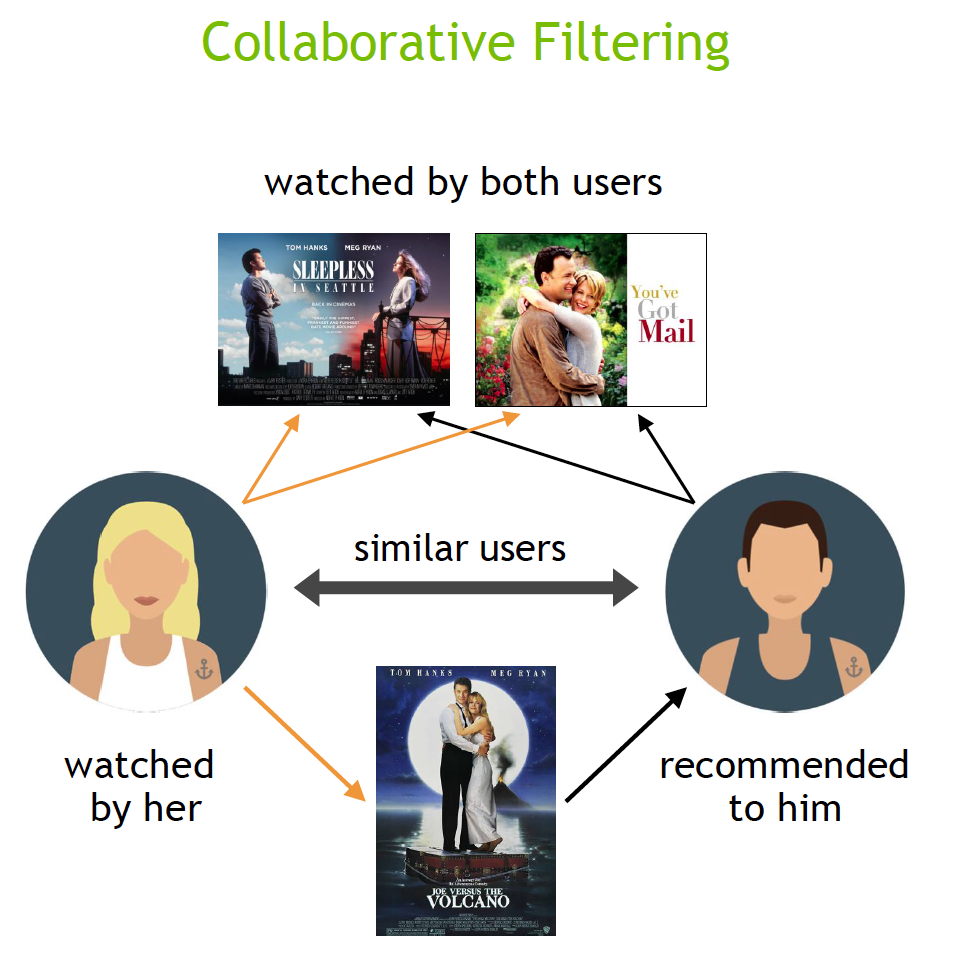
\includegraphics[width=\textwidth]{assets/collaborative_filtering.png}
    \caption{Collaborative Filtering}
    \label{fig:collaborative-filtering}
\end{figure}

\subcaption{Content filtering}\label{subsec:content-filtering}
Content filtering is a technique that uses the features of items a user has interacted with in order to recommend additional items with similar properties. This technique is based on the idea that if a user liked a particular item, he or she will also like an item that is similar to it. 
\begin{figure}[htbp]
    \centering
    \includegraphics[width=\textwidth]{assets/content_filtering.png}
    \caption{Content Filtering}
    \label{fig:content-filtering}
\end{figure}

\subcaption{Hybrid recommendation systems}\label{subsec:hybrid-recommendation-systems}
combine the advantages of the types above to create a more comprehensive recommending system.

\section{Context filtering}\label{sec:context-filtering}
Context filtering is a technique that uses the contextual information of the user by framing the recommendation problem as a contextual multi-armed bandit problem and using the contextual information to learn the user's preferences.
\begin{figure}
    \centering
    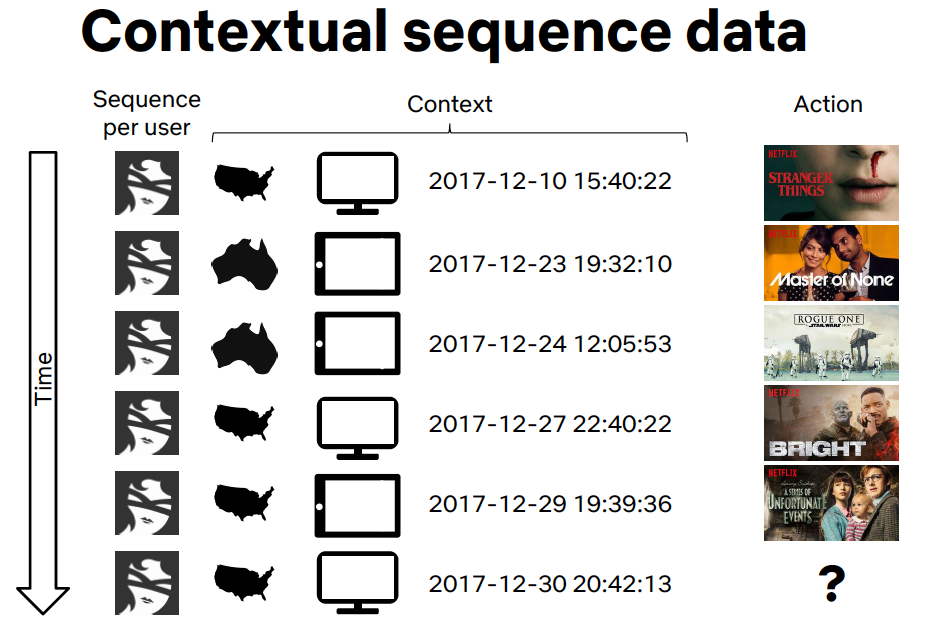
\includegraphics[width=\textwidth]{assets/contextual-sequence-prediction.png}
    \caption{Context Filtering}
    \label{fig:costextual-filtering}
\end{figure}